\documentclass[journal]{IEEEtran}
\ifCLASSINFOpdf
\usepackage[pdftex]{graphicx}
\else
\fi
\usepackage{amsmath}
\usepackage{amssymb}
\usepackage{amsthm}
\usepackage{bm}
\usepackage{mathrsfs}
\hyphenation{La-grange La-grang-ian dy-nam-ics}
\newcommand{\bma}[1]{\left[\begin{array}{#1}}
\newcommand{\ema}{\end{array}\right]}
\newcommand{\trans}{{\ensuremath{\mathsf{T}}}}
\newcommand{\utimes}{ {\raisebox{-0.6ex}{ \kern-1.0ex\raisebox{0.6ex}{ \small $\mathsf{v}$}}} } % 
\newcommand{\onehalf}{\mbox{$\textstyle{\frac{1}{2}}$}}
\DeclareMathAlphabet{\mbf}{OT1}{ptm}{b}{n}
\newcommand{\mbs}[1]{{\boldsymbol{#1}}}
\newcommand{\mbfbar}[1]{{\bar{\mbf{#1}}}}
\newcommand{\mbfhat}[1]{{\hat{\mbf{#1}}}}
\newcommand{\mbftilde}[1]{{\tilde{\mbf{#1}}}}
\newcommand{\mbsbar}[1]{{\bar{\boldsymbol{#1}}}}
\newcommand{\mbshat}[1]{{\hat{\boldsymbol{#1}}}}
\newcommand{\mbstilde}[1]{{\tilde{\boldsymbol{#1}}}}
\newcommand{\pspace}{\mathbb{P}} 
\newcommand{\ura}[1]{{\underrightarrow{{#1}}}}
\newcommand{\vectrix}[1]{\ensuremath \underrightarrow{\boldsymbol{\mathcal{F}}}_{#1}}
\def\fdota{{\raisebox{-2pt}{\LARGE $\cdot$}}}
\def\fdotb{{\raisebox{-0.6ex}{ \kern0.2ex\raisebox{0.8ex}{\tiny $\hspace*{-1ex}\circ$}}}}
\def\fddota{{\raisebox{-2pt}{\LARGE $\cdot\hspace*{-0.2ex}\cdot$}}}
\def\fddotb{{\raisebox{-0.6ex}{ \kern0.2ex\raisebox{0.8ex}{\tiny $\hspace*{-1ex}\circ\circ$}}}}
\newcommand{\fdot}[1]{{^{\fdota{\mbox{\footnotesize${#1}$}}}}}
\newcommand{\fddot}[1]{{^{\fddota{\mbox{\footnotesize${#1}$}}}}}
\newcommand{\beq}{\begin{equation}}
\newcommand{\eeq}{\end{equation}}
\newcommand{\bdis}{\begin{displaymath}}
\newcommand{\edis}{\end{displaymath}}
\newcommand{\beqarray}{\begin{eqnarray}}
\newcommand{\eeqarray}{\end{eqnarray}}
\newcommand{\beqarraynn}{\begin{eqnarray*}}
\newcommand{\eeqarraynn}{\end{eqnarray*}}


\begin{document}

\title{The Dynamics of Some Sort of Interesting System}

\author{Michael~Shell,~\IEEEmembership{Member,~IEEE,}
        John~Doe,~\IEEEmembership{Fellow,~OSA,}
        and~Jane~Doe,~\IEEEmembership{Life~Fellow,~IEEE}
\thanks{M. Shell is with the Department
of Electrical and Computer Engineering, Georgia Institute of Technology, Atlanta,
GA, 30332 USA e-mail: (see http://www.michaelshell.org/contact.html).}
\thanks{J. Doe and J. Doe are with Anonymous University.}
\thanks{Manuscript received April 19, 2005; revised December 27, 2012.}}

\markboth{AER 540 -- Intermediate Dynamics, Fall 2014}
{The Dynamics of Some Sort of Interesting System}

\maketitle

\begin{abstract}
The abstract goes here.
\end{abstract}

\begin{IEEEkeywords}
IEEEtran, journal, \LaTeX, paper, template, AER 540. 
\end{IEEEkeywords}

\IEEEpeerreviewmaketitle

\section{Introduction}

\IEEEPARstart{T}{his} demo file is intended to serve as a ``starter file''
for IEEE journal papers produced under \LaTeX\ using
IEEEtran.cls version 1.8 and later.

I wish you the best of success.

\hfill mds
 
\hfill December 27, 2012 \\

Prof.\ Forbes has modified the template slightly. He's added in some custom commands, shown below, so students use the proper notation. 

Here's some reference, such as the book \cite{book_gabe_glenn} and a paper \cite{paper_shuster_1981}. It is recommend that you use bibtex. Remember, when compiling you must compile in the following order: ``latex bibtex latex latex". 

\subsection{Figures}
\label{sec:figure_section}

This is how you include a figure. See Figure \ref{fig:gimbal}.

\begin{figure}[ht]
    \centering
        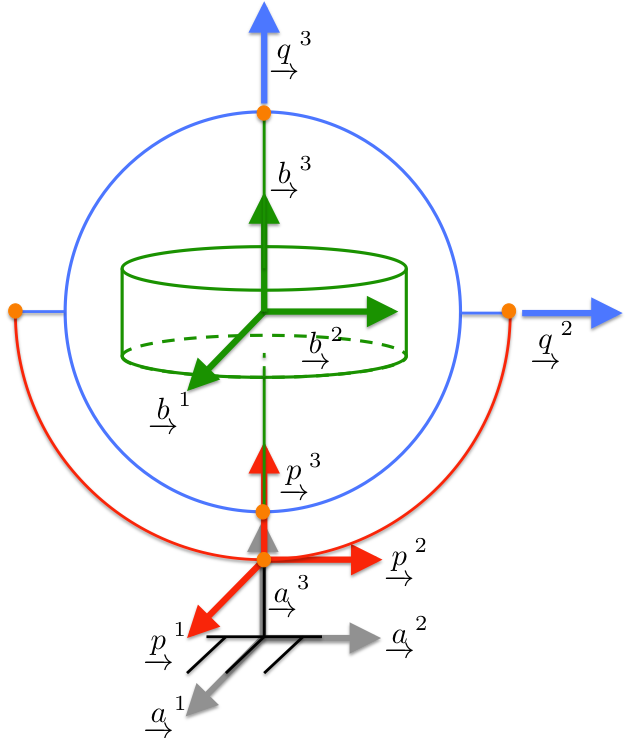
\includegraphics[width=.25\textwidth]{gimbal}
    \caption{This is a gimbal. Make sure your figure captions are descriptive.}
    \label{fig:gimbal}
\end{figure}

\subsection{Custom Latex Commands for AER 540}

A physical vector is an element of physical space:
\beq
	\ura{r} \in \pspace .
	\label{eq:physical_vector}
\eeq
%
The physical vector $\ura{r}$ given in \eqref{eq:physical_vector} can be resolved in any frame, say $\mathcal{F}_a$, as follows:
\bdis
	\ura{r} = \vectrix{a}^\trans \mbf{r}_a . 
\edis
%

Students, please notice how to use ``\texttt{\textbackslash beq}" and ``\texttt{\textbackslash eeq}" along with ``\texttt{\textbackslash label}" both number an equation, and then reference that equation using ``\texttt{\textbackslash eqref}". If you do not need an equation number, then use ``\texttt{\textbackslash bdis}" and ``\texttt{\textbackslash edis}".

The Transport Theorem is
\bdis
	{ \ura{r}^{pq} }^\fdot{a} = { \ura{r}^{pq} }^\fdot{b} + \ura{\omega}^{ba} \times \ura{r}^{pq} 
\edis
%
In $\mathcal{F}_b$ the second term is
\bdis
	{ \mbs{\omega}^{ba}_b }^\times \mbf{r}^{pq}_b .
\edis
Use ``\texttt{\textbackslash mbf}" and ``\texttt{\textbackslash mbs}" properly. Also, use ``$(\cdot)^\times$" properly.  
The acceleration of point $p$ relative to point $q$ with respect to $\mathcal{F}_a$ is
\bdis
	{\ura{r}^{pq}}^{\fddot{a}} ,
\edis
and the acceleration of point $p$ relative to point $q$ with respect to $\mathcal{F}_b$ is
\bdis
	{\ura{r}^{pq}}^\fddot{b} .
\edis

The column matrix $\mbf{r}_a$ can be written as
\beqarraynn
	\mbf{r}_a
	& = &
	\bma{c}
		r_{a,1} \\
		r_{a,2} \\
		r_{a,3}
	\ema \\
	& = &
	r_{a,1}
	\bma{c}
		1 \\
		0 \\
		0
	\ema
	+
	r_{a,2}
	\bma{c}
		0 \\
		1 \\
		0
	\ema
	+
	r_{a,3}
	\bma{c}
		0 \\
		0 \\
		1
	\ema .
\eeqarraynn
%
A general matrix can be written as
\bdis
	\mbf{A} 
	=
	\bma{cc}
		1 & 2 \\
		4 & 9
	\ema .
\edis
%
A matrix of matrices can also be written:
\bdis
	\mbf{P}
	=
	\bma{ccc}
		\mbf{A} & \mbf{B} & \mbf{C} \\
		\mbf{D} & \mbf{E} & \mbf{F} \\
		\mbf{G} & \mbf{H} & \mbf{I} \\
	\ema .
\edis

You can refer to previous sections, such as Section \ref{sec:figure_section}.

A matrix differential equation is
\bdis
	\mbf{M} \ddot{\mbf{q}} + \mbf{K} \mbf{q} = \mbf{0} .
\edis

\subsection{Lists}
We can write numbered lists:
\begin{enumerate}

\item This is an item.

\item This is another item. 

\end{enumerate}

\subsubsection{Subsubsection Heading Here}
Subsubsection text here.

\section{Conclusion}
The conclusion goes here.

\appendices
\section{Proof of the First Zonklar Equation}
Appendix one text goes here.

\section{}
Appendix two text goes here.

\section*{Acknowledgment}


The authors would like to thank...

\ifCLASSOPTIONcaptionsoff
  \newpage
\fi

\bibliographystyle{IEEEtran}

\bibliography{540_refs}

\begin{IEEEbiography}{Michael Shell}
Biography text here.
\end{IEEEbiography}

\begin{IEEEbiographynophoto}{John Doe}
Biography text here.
\end{IEEEbiographynophoto}

\begin{IEEEbiographynophoto}{Jane Doe}
Biography text here.
\end{IEEEbiographynophoto}

\end{document}


